\section{Applications of EM: Unsupervised Classification}
\begin{definition}[Unsupervised Classification]
    Given data vectors $\mathbf{x}_1,\mathbf{x}_2,\dots,\mathbf{x}_n\in\R^d$ and a set of possible classes $\mathcal{C}=\{1,2,\dots,k\}$, we attempt to find $z_1,z_2,\dots,z_n\in \mathcal{C}$ and parameters $\theta$ such that $\prod_{i=1}^n p(\mathbf{x}_i,z_i;\theta)$. In other words, the MLE under a known distribution type is maximized.
\end{definition}
This definition can seen as a reformulation of the ``Distribution Learning with Hidden Latent Variables'' where $\mathbf{z}_i$ is limited to a discrete set. By solving for $q$ with EM, we're able to derive the MLE for the classes $z_i$ as follows
\begin{align*}
    \hat{z} 
    &= \arg\max_{z\in\mathcal{C}} p(z|\mathbf{x};\theta) \\
    &= \arg\max_{z\in\mathcal{C}} \frac{p(\mathbf{x}|z;\theta)p(z)}{p(\mathbf{x})} & \text{Bayes' Rule}\\
    &= \arg\max_{z\in\mathcal{C}} p(\mathbf{x}|z;\theta)p(z) & p(\mathbf{x})\text{ is constant} \\
    &= \arg\max_{z\in\mathcal{C}} p(\mathbf{x}|z;\theta)\hat{q}(z) & \hat{q}\text{ is an estimate of the prior}
\end{align*}

\subsection{K-means Clustering}
The K-means clustering algorithm \cite{kmeans} finds an estimate to the unsupervised classification problem using the following procedure. First assign centroids $\boldsymbol{\mu}_j^{(0)}$ for $j=\{1,2,\dots,k\}$ to random points. Until convergence, run
\begin{itemize}
    \item $\mathcal{S}_j^{(t)} = \{i\in\{1,2,\dots,n\}:j=\arg\max_l\|\boldsymbol{\mu}_l^{(t)}-\mathbf{x}_i\|_2^2\}$
    \item $\boldsymbol{\mu}_j^{(t+1)}=\frac{1}{|\mathcal{S}_j^{(t)}|}\sum_{i\in \mathcal{S}_j^{(t)}} \mathbf{x}_i$
\end{itemize}
Finally, assign $\hat{z}_i=\arg\min_j\|\boldsymbol{\mu}_j^{(t)}-\mathbf{x}_i\|_2^2$. We will first argue that the algorithm above can be seen as a special case of the EM algorithm. Consider a simpler case of the Gaussian Mixture problem such that:
\begin{itemize}
    \item For $j=\{1,2,\dots,k\}$, $\phi_j=\frac{1}{k}$ (each cluster has an equal chance of being assigned)
    \item For $j=\{1,2,\dots,k\}$, $\Sigma_j=\sigma^2\mathbf{I}_{d\times d}$, this value of $\sigma$ will be clarified later.
\end{itemize}
Knowing $\phi_j$, we are able to simply the E-step as follows:
\[
    q_i^{(t)}(z) = p(z|\mathbf{x}_i;\theta^{(t)}) = \frac{p(\mathbf{x}_i,z;\theta^{(t)})}{\sum_{j=1}^k p(\mathbf{x}_i,j;\theta^{(t)})} = \frac{\exp(-\|\mathbf{x}_i-\boldsymbol{\mu}^{(t)}_z\|_2^2/2\sigma^2)}{\sum_{j=1}^k \exp(-\|\mathbf{x}_i-\boldsymbol{\mu}_j\|_2^2/2\sigma^2)}
\]
the next trick involves taking the limit of $\sigma\to0$, which implies that each Gaussian cluster converges to an impulse function. This is also called \textbf{hard-labeling}. We could simply to the final term as $1/\sigma$ dominates in the term where $\|\mathbf{x}_i-\boldsymbol{\mu}^{(t)}_j\|_2^2$ is smallest.
\[
\lim_{\sigma\rightarrow0} q_i^{(t)}(z) = \lim_{\sigma\rightarrow0} \frac{\exp(-\|\mathbf{x}_i-\boldsymbol{\mu}^{(t)}_z\|_2^2/2\sigma^2)}{\sum_{j=1}^k \exp(-\|\mathbf{x}_i-\boldsymbol{\mu}^{(t)}_j\|_2^2/2\sigma^2)} = \begin{cases}
    1 & z = \arg\min_j\|\boldsymbol{\mu}_j^{(t)}-\mathbf{x}_i\|_2^2 \\
    0 & \text{otherwise}
\end{cases}
\]
substituting to the M-step $\boldsymbol{\mu}_z^{(t)} = \frac{\sum_{i=1}^n q_i^{(t)}(z) \mathbf{x}_i}{\sum_{i=1}^n q_i^{(t)}(z)}$: defining $\mathcal{S}_j^{(t)} = \{i\in\{1,2,\dots,n\}:j=\arg\max_l\|\boldsymbol{\mu}_l^{(t)}-\mathbf{x}_i\|_2^2\}$ like above,
\[
    \boldsymbol{\mu}_z^{(t)} = \frac{1}{|\mathcal{S}_j^{(t)}|}\sum_{i\in \mathcal{S}_j^{(t)}} \mathbf{x}_i
\]
which agrees with expression presented in the K-means Clustering algorithm. As such, as a direct result of the EM Algorithm Convergence theorem, the K-means Clustering guarantees that the log-likelihood decreases monotonically in time.

\subsection{Gaussian Mixture Classification}
As expressed in the beginning of this section, we are able to express the MLE for the label as such:
\begin{align*}
    \hat{z}_i
    &= \arg\max_z p(\mathbf{x}_i|z;\theta)\hat{q}(z) \\
    &= \arg\max_z \frac{\phi_z}{|\Sigma_z|^{1/2}} \exp\left(\frac{\|\mathbf{x}_i-\boldsymbol{\mu}_z\|^\top\Sigma_z^{-1}\|\mathbf{x}_i-\boldsymbol{\mu}_z\|}{2}\right)
\end{align*}
\subsection{Comparison}
The Gaussian Mixture method generalizes K-means Clustering with the following distinction
\begin{itemize}
    \item \textbf{Soft-labeling}: the Gaussian Mixture model considers the probability of each cluster having distinct spread, and that all points have a possibility of being a tail outlier from a faraway cluster.
    \item \textbf{Cluster probability}: as a direct consequently of hard-labeling, the K-means Clustering algorithm is unable to produce a distribution-type posterior probability $p(z|\mathbf{x}_i;\theta^{(t)})$, while the Gaussian Mixture method naturally produces this value.
\end{itemize}
Still, both model both utilizes the Gaussian Distribution to model the associated cluster and apply the EM Algorithm to solve for an MLE estimate. As such, both models suffer greatly from poorly initialized $\boldsymbol{\mu}_j$ centroids as their convergence only guarantees up to the monotonic decrease of the loss function, leading to local minima situations. To visualize this, we first generate sampled Gaussian Mixture data from $\R^2$ as shown in \ref{fig:clusters}. Implementations can be found in \texttt{code/unsupervised-classification.ipynb}.
\begin{figure}[h]
    \centering
    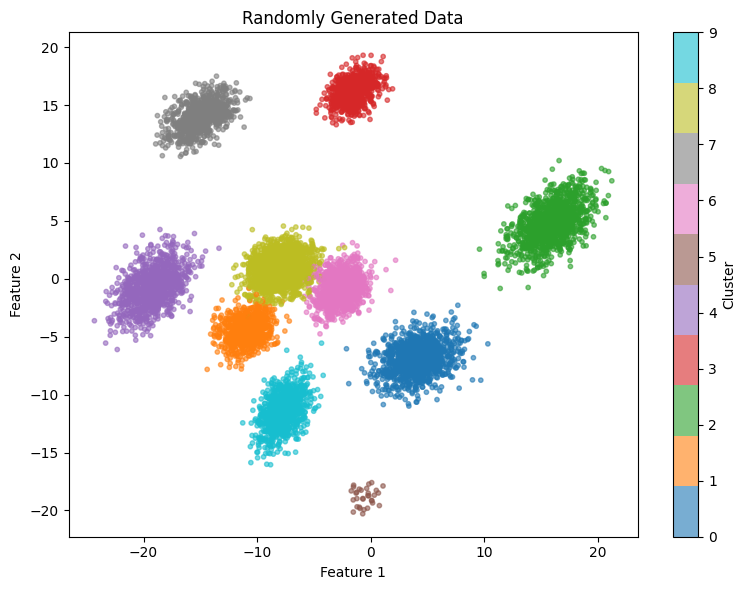
\includegraphics[width=0.6\linewidth]{figures/cluster-gt.png}
    \caption{Randomly Generated Cluster Data}
    \label{fig:clusters}
\end{figure}

We first discuss the results from K-means clustering in figure \ref{fig:kmeans}. We notice a poor accuracy in classes 2 and 3 as a result of these two predicted clusters ``inhabiting'' on of the original clusters. Due to starting points being sampled from the dataset itself, it is possible that the class 2 and 3 centroids are originally picked from this cluster and aren't able to be separated due to local optima. While Gaussian Mixture models (see figure \ref{fig:gmm}) is shown to obtain a higher performance, we notice that Gaussian Mixture fitting also suffers from the same problem (class 9 in the figure). Still, the incorporation of prior terms in Gaussian Mixture models is able to improve its accuracy over K-means (these implementations all use the same seed and starting points).

\begin{figure}[h]
    \centering
    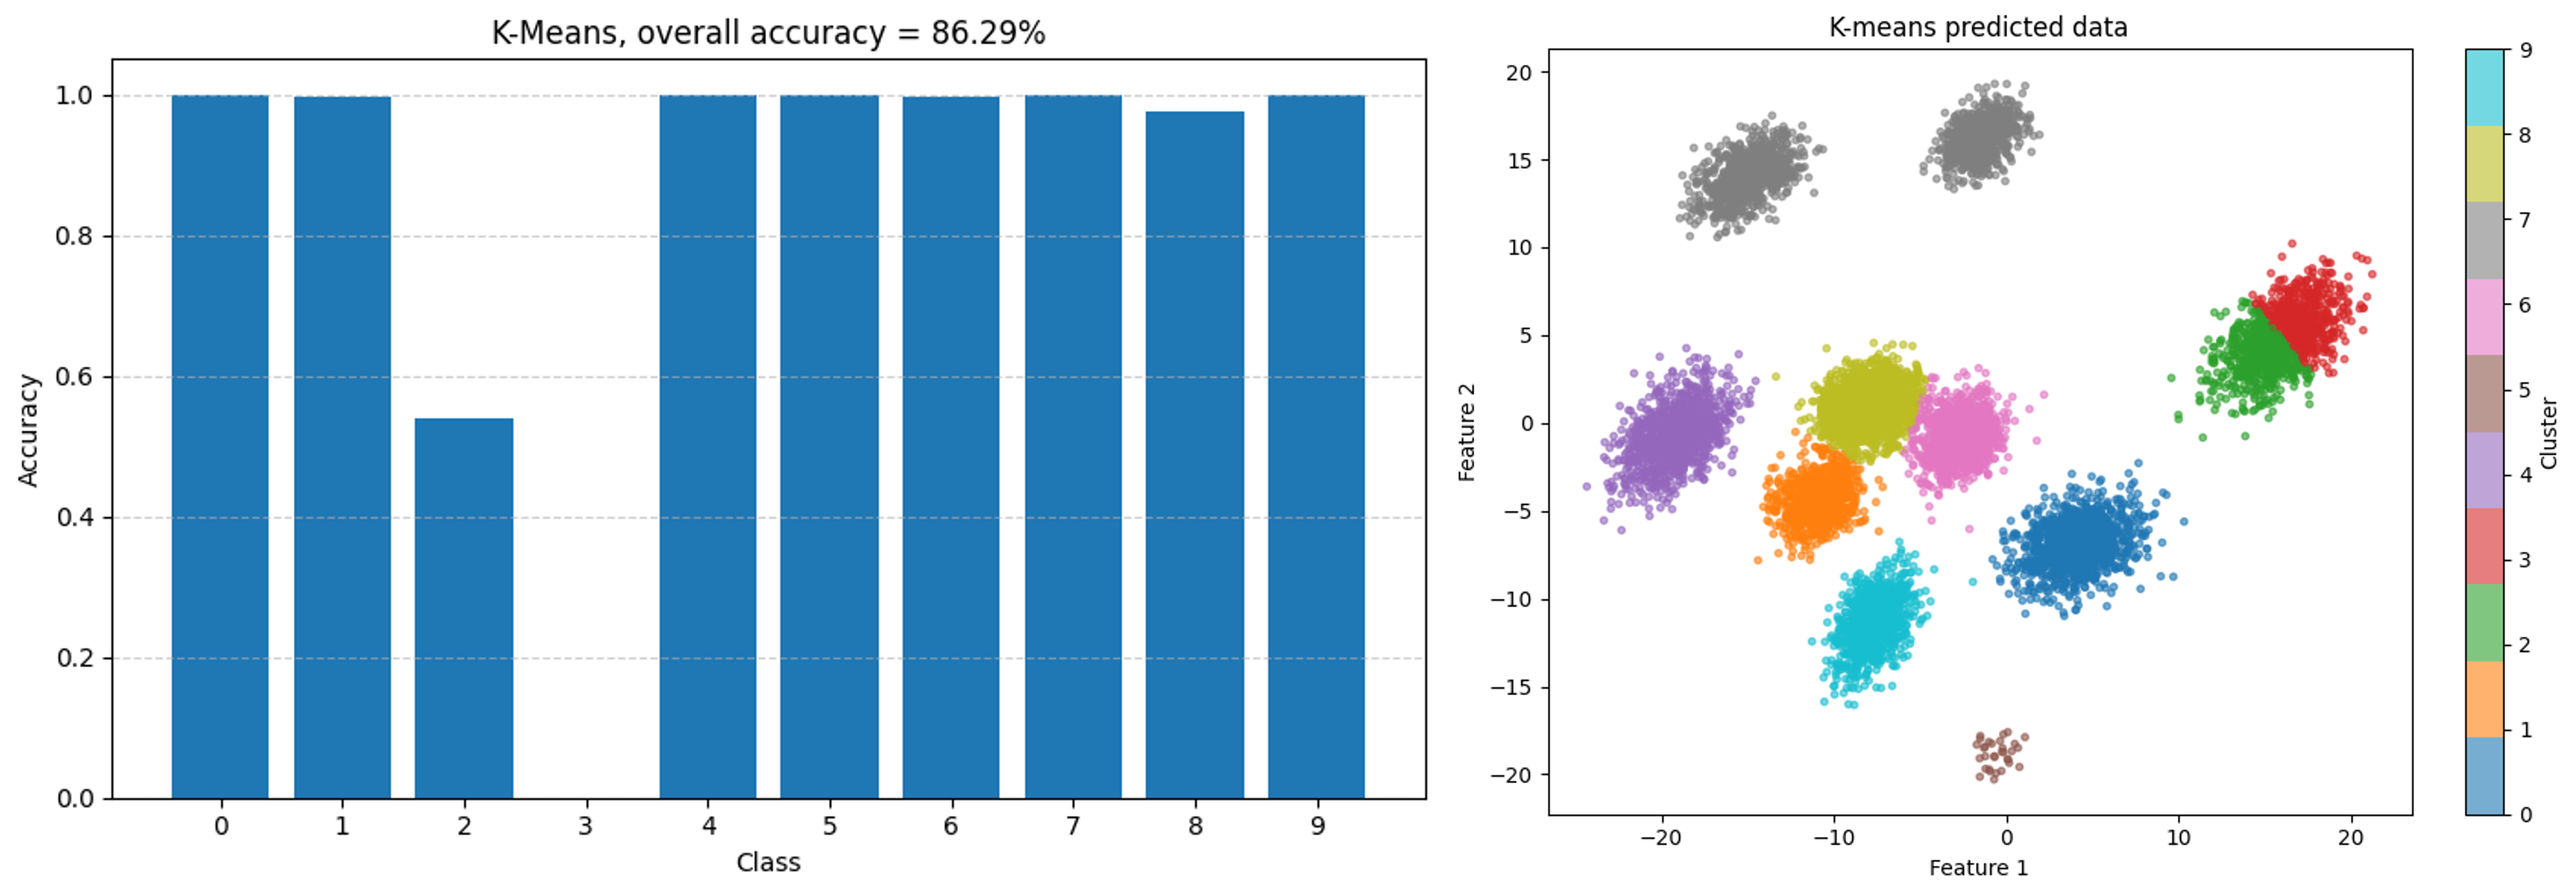
\includegraphics[width=0.9\linewidth]{figures/result-kmeans.png}
    \caption{K-Means Clustering Results}
    \label{fig:kmeans}
\end{figure}

\begin{figure}[h]
    \centering
    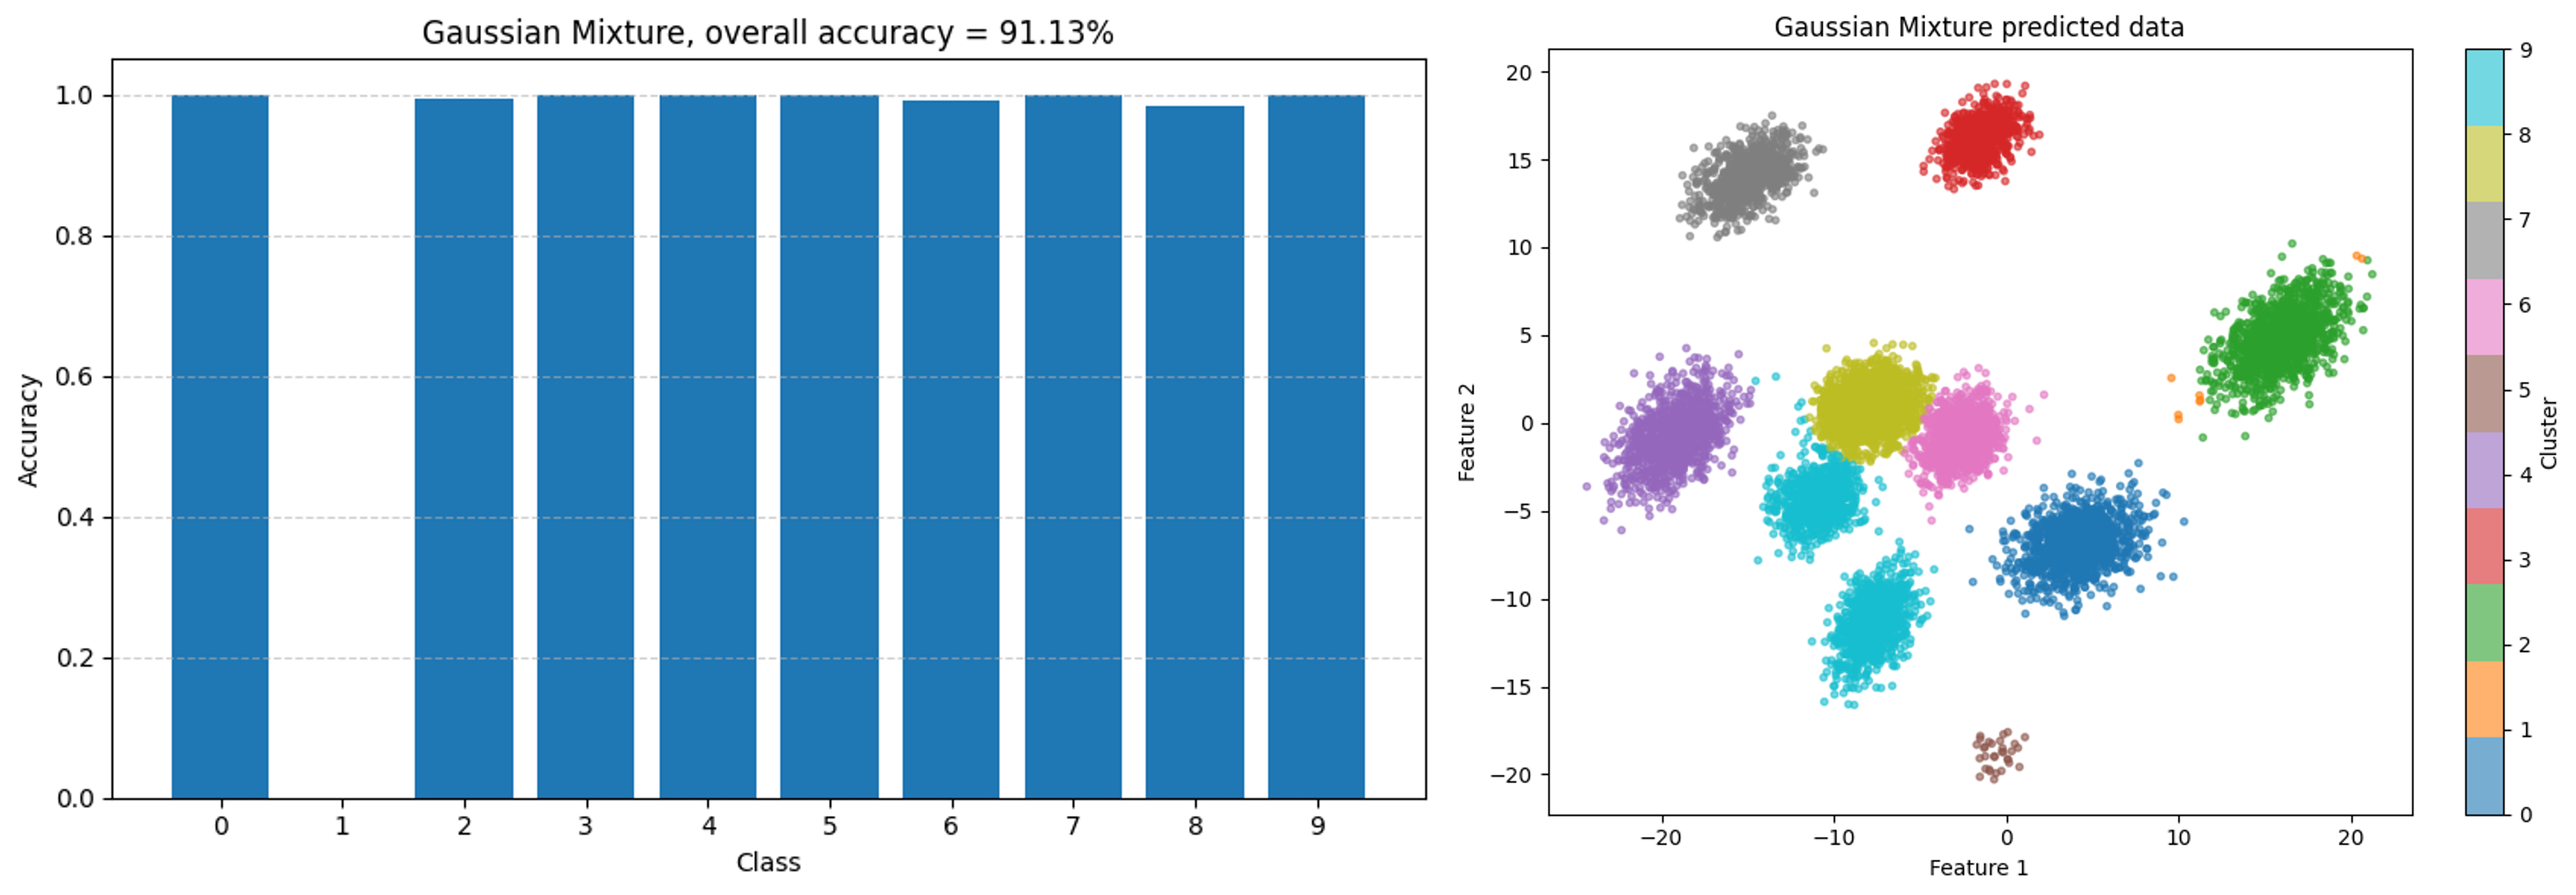
\includegraphics[width=0.9\linewidth]{figures/result-gmm.png}
    \caption{Gaussian Mixture Clustering Results}
    \label{fig:gmm}
\end{figure}